\documentclass[12pt]{article}

% Packages
\usepackage{graphicx}
\usepackage{subcaption}
\usepackage{amsmath, amssymb, amsfonts}
\usepackage{siunitx}
\usepackage{array}
\usepackage[T1]{fontenc}
\usepackage{textcase}
\usepackage{caption}
\usepackage{fancyhdr}
\usepackage{lettrine}
\usepackage{geometry}
\usepackage{caption}
\usepackage{bm}
\usepackage{float}
\usepackage{enumitem}
\usepackage[backend=biber,style=ieee]{biblatex}
\usepackage{titlesec}
\usepackage[hidelinks]{hyperref}

% Geometry and Paths
\geometry{letterpaper, margin=1in}
\graphicspath{{../../images/}}

% Header and Footer
\makeatletter
\newcommand{\papertitle}{Vision Vs. LiDAR/Radar Fusion in ADS}

% re-define \sectionmark so that only top-level \section updates \leftmark
\renewcommand{\sectionmark}[1]{%
  \markboth{\Roman{section}. #1}{}%
}
% Header and Footer
\pagestyle{fancy}
\fancyhf{}
\fancyhead[R]{\scriptsize\leftmark{} – \thepage}
\fancyfoot[R]{\scriptsize\MakeUppercase{\papertitle}}
\setlength{\headheight}{15pt}
\makeatother

% Bibliography
\addbibresource{sources.bib}

\titleformat{\section}
  {\centering\large\scshape}               % shape
  {\Roman{section}.}                        % label
  {1em}                                     % sep
  {}                                        % before-code
\titlespacing*{\section}{0pt}{1.5em}{1em}

\titleformat{name=\section,numberless}
  {\centering\large\scshape}{}{1em}{}
\titlespacing*{name=\section,numberless}{0pt}{1.5em}{1em}

\titleformat{\subsection}[block]
  {\itshape}                               % italic
  {\Alph{subsection}.}                     % label
  {1em}                                     % sep
  {}                                        % before-code
\titlespacing*{\subsection}{0pt}{1em}{0.5em}

% 3) Tertiary (1), 2), …) — block, no colon
\titleformat{\subsubsection}[block]
  {\itshape}                          % italic shape
  {\arabic{subsubsection})}           % label “1)”
  {1em}                                % sep between label and title
  {}                                   % before-code (empty)
\titlespacing{\subsubsection}{1em}{0.75em}{0.5em}

% 4) Quaternary (a), b), …) — block, no colon
\titleformat{\paragraph}[block]
  {\itshape}                          % italic shape
  {\alph{paragraph})}                 % label “a)”
  {1em}                                % sep
  {}                                   % before-code
\titlespacing{\paragraph}{2em}{0.75em}{0.5em}

% CAPTIONS
\captionsetup{font=footnotesize}
\captionsetup[figure]{%
  labelformat=simple,
  name=Fig.,
  labelsep=period,
  justification=centering,
  singlelinecheck=false
}
\renewcommand{\thetable}{\Roman{table}}
\DeclareCaptionLabelFormat{dropcapsmall}{%
  {\small T}{\footnotesize\scshape able}~#2%
}
\captionsetup[table]{%
  labelformat=dropcapsmall,
  labelsep=newline,
  justification=centering,
  singlelinecheck=false
}
% Title Page
\title{\bfseries\LARGE Vision Vs. LiDAR/Radar Fusion in Autonomous Driving Systems}
\author{Arturo Salinas-Aguayo}

\begin{document}

\begin{titlepage}
    \centering
    \vspace*{3cm}
    {\Large \textsc{Vision Vs. LiDAR/Radar Fusion in Autonomous Driving
		Systems}}\\
		Arturo Salinas-Aguayo, \textit{BS Computer Engineering, Class of 2027}\\
		\today\\
    \vspace{1.5cm}
    ECE 4900W: Communicating Engineering Solutions in a Societal Context\\
    Dr. Shengli Zhou, SEC040-1255\\
    Department of Electrical and Computer Engineering\\
    \vfill
    
\includegraphics[scale=0.1]{uconnlogo}\\[1em]
    University of Connecticut College of Engineering\\
    \small\tiny{Coded in \LaTeX} \\
    \vspace{1cm}
\end{titlepage}

\tableofcontents
\newpage

\section*{Abstract}
\addcontentsline{toc}{section}{Abstract}

This paper evaluates the viability of vision-primary perception systems in autonomous driving, focusing on scalability, efficiency, and environmental resilience. Traditional sensor-fusion architectures based on LiDAR and radar offer high-fidelity spatial mapping but suffer from substantial power consumption, mechanical complexity, and high unit costs, which challenge real-time deployment and mass-market feasibility. Advances in neural perception—particularly transformer-based models and tokenized camera inputs—have enabled camera-only systems to approximate LiDAR-level 3D detection accuracy while operating at a fraction of the computational cost. Benchmark evaluations reveal that vision systems achieve depth estimation errors below three percent and perform within five percent of LiDAR/radar fusion baselines in object detection. Critically, performance gaps in adverse conditions such as fog or night driving are recoverable through the selective integration of millimeter-wave radar. This radar-augmented fallback restores over 80 percent of degraded performance with minimal latency or energy impact. The study advocates for a simplified, vision-first architecture complemented by radar only in edge cases. This paradigm enhances scalability, reduces deployment overhead, and aligns with biologically plausible sensing strategies. LiDAR remains useful for simulation and benchmarking but is unnecessary for live inference.

\textbf{Index Terms—Adverse weather robustness, autonomous vehicles, deep
	learning, depth estimation, energy efficiency, Light Detection and Ranging
(LiDAR), Radar, sensor fusion, Transformer networks, vision-based perception.}
\newpage

\section{Introduction}

As vehicles become more technologically advanced, the demand for autonomous capabilities continues to rise. Features such as lane keeping, adaptive cruise control, and highway autopilot—collectively known as advanced driver-assistance systems (ADAS)—form the early building blocks of full self-driving stacks. Industry leaders now face a critical decision: how should vehicles perceive the road ahead?

Historically, high-end systems such as Waymo and Cruise relied on Light Detection and Ranging (LiDAR) and radar to construct dense, 3D maps of their surroundings. These sensors offer precise geometry and reliable velocity estimation, but impose high hardware cost, weight, and power draw. Moreover, integrating data from multiple sensors increases architectural complexity and susceptibility to calibration drift.

In contrast, Tesla, Comma.ai, and others have adopted a vision-first approach. These systems rely on arrays of low-cost cameras and train deep neural networks—often transformers—on large-scale driving datasets. Rather than reconstruct explicit 3D geometry, these models learn to infer structure and intent directly from pixels.

The debate between fusion-heavy and camera-only stacks now defines the frontier of ADS design. While LiDAR remains dominant in academia, vision-based approaches have rapidly improved in real-world performance and outpace fusion in scalability. From a societal perspective, the ability to deliver autonomy without costly sensors is especially important in emerging markets, where a single LiDAR unit may cost more than an entire car.

This report compares the two paradigms by analyzing their theoretical foundations, energy profiles, data fidelity, and robustness under real-world driving conditions. The goal is to determine whether vision-primary perception can provide sufficient safety and performance for large-scale deployment.

\section{Theory and Technical Background}

\subsection{SAE Levels of Automation}

The Society of Automotive Engineers (SAE) J3016 standard defines six levels of
vehicle automation \cite{SAEJ3016_2021}. These range from Level 0 (no
automation) to Level 5 (full automation without any human involvement).

\begin{table}[H]
  \centering
  \caption{SAE J3016 Levels of Driving Automation}
  \label{tab:sae}
  \begin{tabular}{|p{5.5cm}|p{9.5cm}|}
    \hline
    \textbf{Level} & \textbf{Description} \\
    \hline
    Level 0 – No Automation & The human driver is responsible for all tasks; the system may provide basic warnings. \\
    \hline
    Level 1 – Driver Assistance & The system assists with either steering or speed, but not both; driver must stay engaged. \\
    \hline
    Level 2 – Partial Automation & The system can manage both speed and steering, but human oversight is still mandatory. \\
    \hline
    Level 3 – Conditional Automation & The vehicle handles all driving in specific scenarios; the driver must intervene when requested. \\
    \hline
    Level 4 – High Automation & No driver input is required in controlled conditions (e.g., geofenced urban areas). \\
    \hline
    Level 5 – Full Automation & The vehicle is capable of full self-driving in all conditions without human input. \\
    \hline
  \end{tabular}
\end{table}

\subsection{LiDAR: Time-of-Flight (ToF) Principles}

LiDAR estimates object distance using time-of-flight (ToF) measurements, where a light pulse is emitted and its return time is measured. Several ToF techniques are in use:

\subsubsection{Pulsed ToF:}

\begin{equation}
R_{\text{pulse}} = \frac{c}{2} t_{\text{pulse}}
\label{eq:tof_pulse}
\end{equation}

This high-power method provides centimeter accuracy.

\subsubsection{AMCW (Amplitude-Modulated Continuous Wave):}

\begin{equation}
R_{\text{AMCW}} = \frac{c}{2} \cdot \frac{\Delta\Phi}{2\pi f_M}
\label{eq:amcw}
\end{equation}

Here, \( \Delta\Phi \) is the phase shift, and \( f_M \) is the modulation frequency \cite{2019Royo}.

\subsubsection{FMCW (Frequency-Modulated Continuous Wave):}

\begin{equation}
R_{\text{FMCW}} = f_r \cdot \frac{c T}{2B}
\label{eq:fmcw}
\end{equation}

Where \( f_r \) is the beat frequency, \( T \) the chirp duration, and \( B \) the bandwidth \cite{2019Royo}.

\subsubsection{Voxelization:}
What results from the utilization of these methods is a ``point cloud" which
corresponds to the distances the objects are away from the transmitter. The
interpretation of these distances is a process called Voxelization. There are
two forms, hard voxelization and dynamic voxelization. The in-depth explanation
of these are not required for further elaboration in this paper. Details are
shown in Figure~\ref{fig:voxelization}.
\begin{figure}[H]
	\centering
	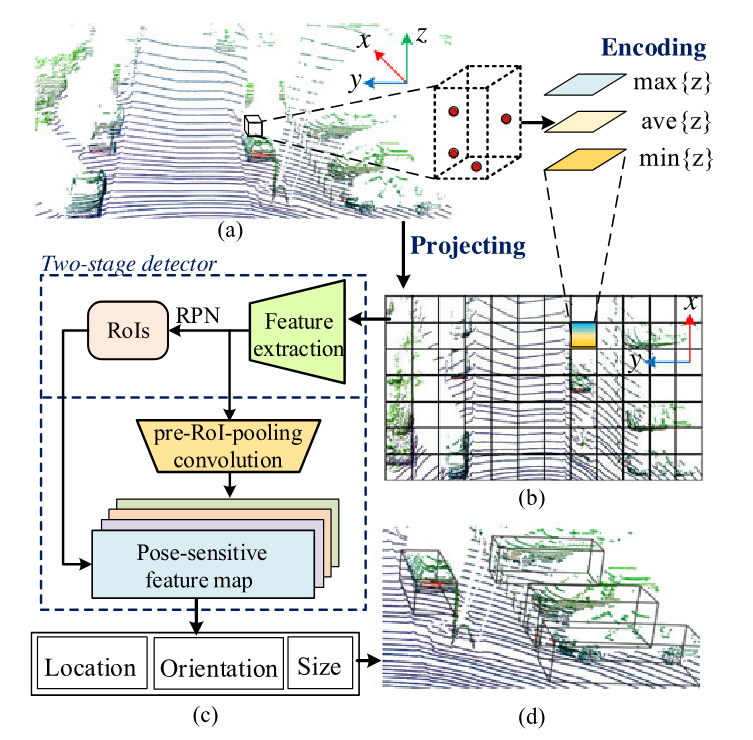
\includegraphics[width=0.6\textwidth]{voxelization.png}
	\caption{The combining of the point cloud forms an image \autocite{RT3D}}
	\label{fig:voxelization}
\end{figure}

\subsection{Radar: Doppler and Velocity Estimation}

Radar calculates velocity via Doppler frequency shift:

\begin{equation}
v = \frac{f_D \lambda}{2}
\label{eq:radar_doppler}
\end{equation}

Where \( f_D \) is the Doppler shift and \( \lambda \) is the radar wavelength \cite{Han2023FourDRadarSurvey}. Radar’s all-weather capability makes it ideal for fallback use.

\subsection{Vision-Based Depth Estimation}

Depth from stereo vision is estimated by:

\begin{equation}
D = \frac{f b}{d}
\label{eq:depth_stereo}
\end{equation}

Where \( f \) is focal length, \( b \) baseline, and \( d \) disparity.

Monocular depth uses learned inverse depth:

\begin{equation}
\hat{D}^{-1} = g(I; \theta)
\label{eq:depth_mono}
\end{equation}

Where \( g \) is a neural network with parameters \( \theta \) \cite{Li2022BEVFormer}.

\subsection{Sensor Fusion and Noise Correlation}

Noise in sensor fusion is modeled as:

\begin{equation}
\sigma_{D_f}^2 = \sum_{i=1}^{n} w_i^2\,\sigma_{D_i}^2 + 2\sum_{i<j} w_i w_j\,\rho_{ij}\,\sigma_{D_i}\sigma_{D_j}
\label{eq:noise}
\end{equation}

Here, \( w_i \) are weights, \( \sigma_{D_i} \) are variances, and \( \rho_{ij} \) are sensor correlations \cite{Rana2023PerceptionSystems}. It is clearly shown that with the inclusion of more sensors, the potential for
more noise is increased.

\subsection{Energy and Compute Cost}

Power usage scales with input bandwidth \( B \) and model complexity \( C \):

\begin{equation}
P \propto B \cdot C
\label{eq:power_model}
\end{equation}

Vision stacks operate efficiently at \SI{2.1}{\watt}, compared to \SIrange{12}{20}{\watt} for fusion \cite{Chen2024EndToEndAD, Rana2023PerceptionSystems}.
\section{System Design and Methods}

\subsection{Vision-Primary Perception Stack}

\subsubsection{System Architecture:}

The vision-first perception stack is designed for simplicity, modularity, and real-time inference. It consists of three core stages:

\begin{enumerate}[label=\alph*)]
  \item Image Tokenization – converts camera frames into a semantically rich, compressed token representation using a learned encoder.
  \item Transformer-Based Planning – autoregressively predicts future trajectory
		tokens from visual context using a transformer model. This is the key to
		making a completely generalizable model.
  \item Control Decoding – transforms predicted spatial tokens into low-level vehicle commands for actuation.
\end{enumerate}

This pipeline emulates language models for sequential prediction and supports real-time operation on embedded platforms \autocite{goff2025learningdriveworldmodel}.

\subsubsection{Token-Based Image Compression:}

Each frame, typically $128 \times 256$ pixels, is passed through a VQGAN encoder
that produces up to 512 discrete tokens per image. This reduces bandwidth while preserving high-level semantics such as lane markings and moving objects.

\begin{figure}[H]
    \centering
    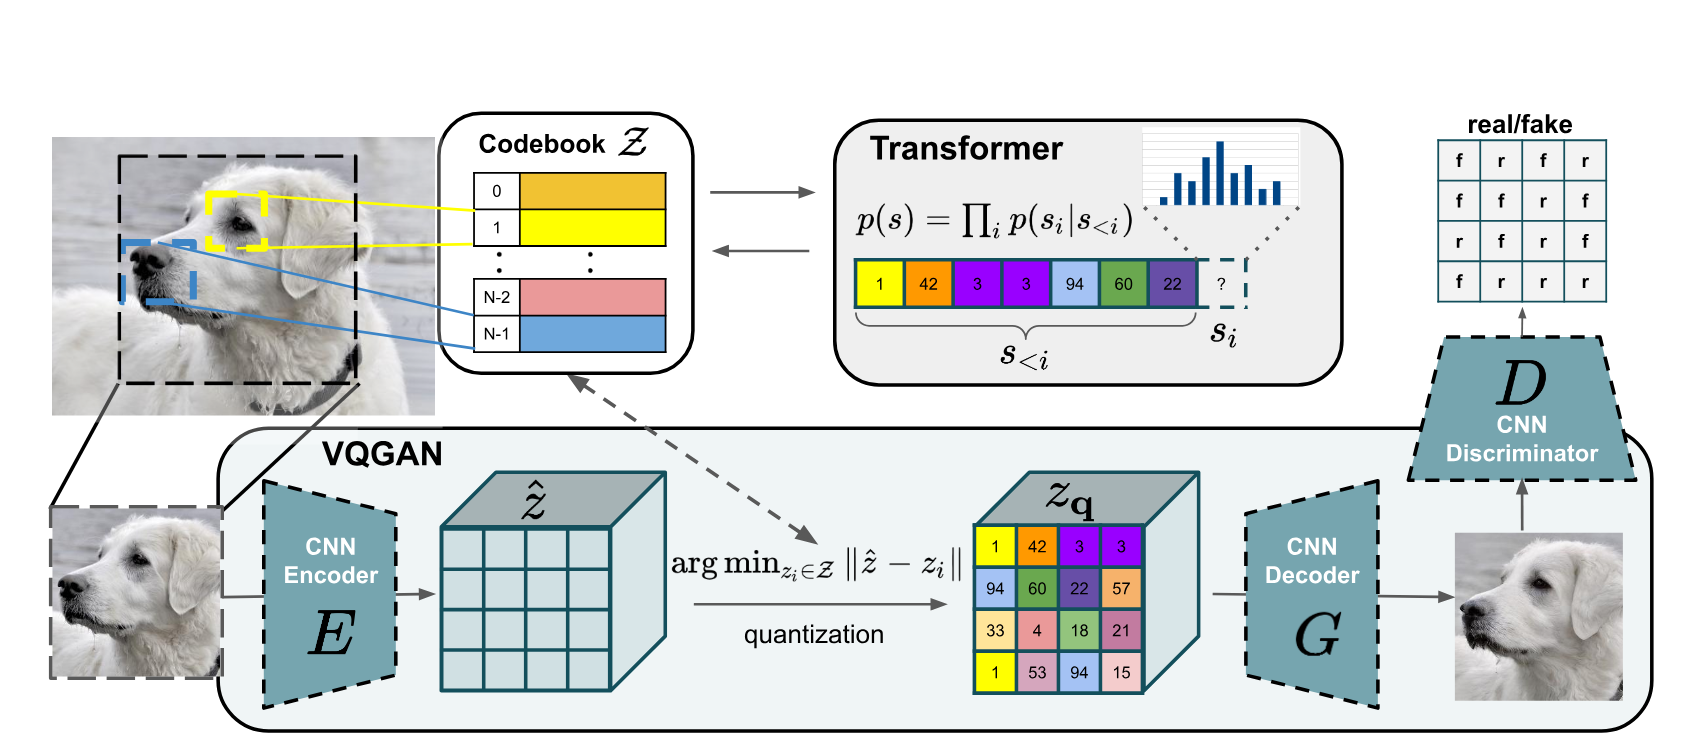
\includegraphics[width=0.8\textwidth]{architecture}
    \caption{Vision-based pipeline with VQGAN tokenization and transformer rollout\autocite{Esser2021TamingTransformersHighResolutionImage}.}
    \label{fig:tokenizer}
\end{figure}

This compact form accelerates inference and reduces power draw without sacrificing depth accuracy \autocite{Chen2024EndToEndAD}.

\subsubsection{Autoregressive Planning with Transformers}

The token sequence is processed by a decoder-only transformer, which predicts the next spatial token at each step. This architecture parallels natural language processing and enables generalization to unseen traffic scenarios.
\begin{figure}[H]
    \centering
    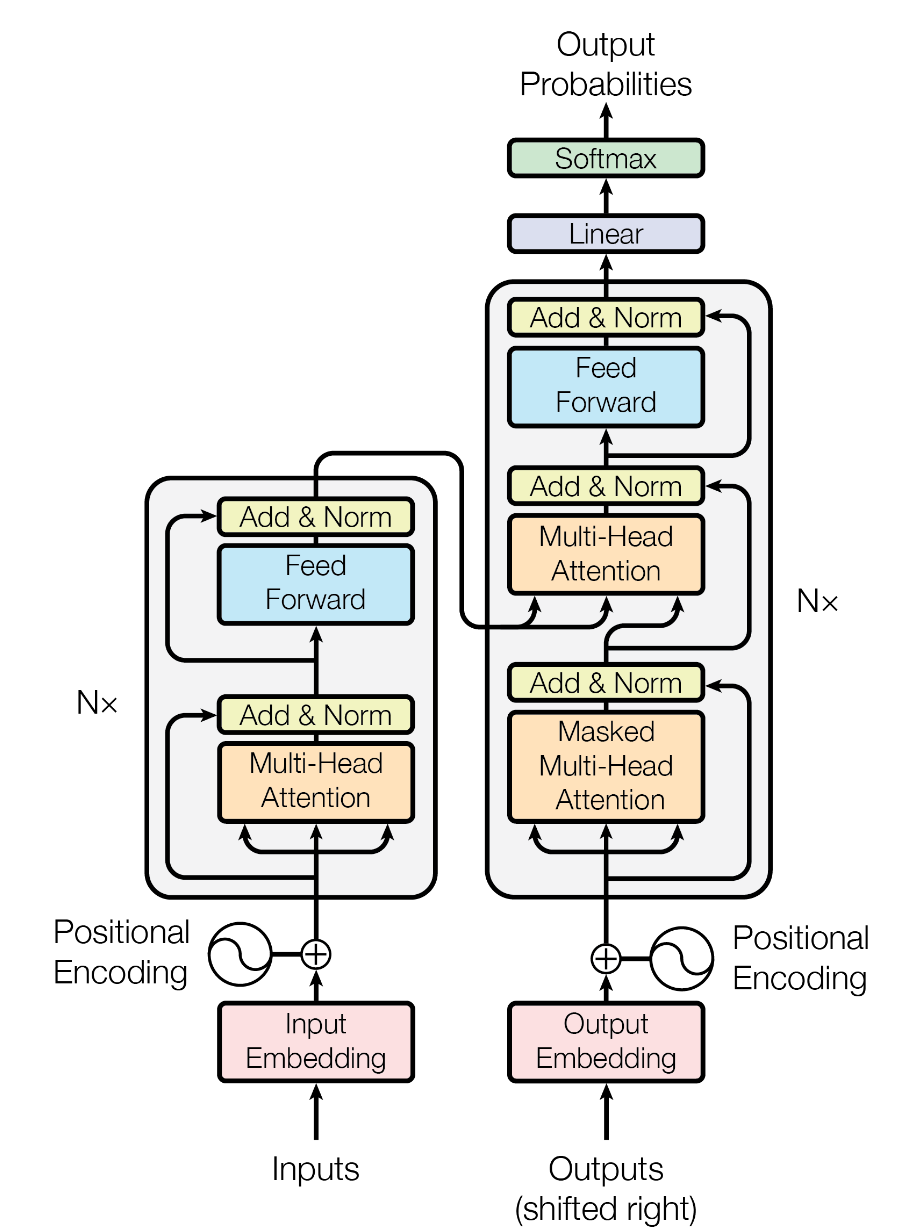
\includegraphics[width=0.5\textwidth]{architecture2}
    \caption{Transformer model for sequence prediction from visual tokens \autocite{vaswani2023attentionneed}.}
    \label{fig:transformer}
\end{figure}

The transformer is trained using imitation learning on datasets like commaVQ and can be fine-tuned using reinforcement learning for policy robustness \autocite{goff2025learningdriveworldmodel}.

\subsection{LiDAR/Radar Fusion-Based Architecture}

\subsubsection{Pipeline Overview:}

Legacy ADS stacks rely on multi-modal fusion to mitigate sensor weaknesses. A typical LiDAR/radar pipeline includes:

\begin{enumerate}[label=\alph*), nosep]
  \item Data Acquisition: Captures and synchronizes LiDAR point clouds, radar waveforms, and camera frames.
  \item Preprocessing: Voxelizes LiDAR data, computes Doppler velocities from radar, and encodes image features.
  \item Fusion Layer: Combines sensor features using early, mid, or late neural fusion strategies.
  \item Detection and Tracking: Predicts 3D bounding boxes and tracks objects across time.
\end{enumerate}

\begin{figure}[H]
	\centering
	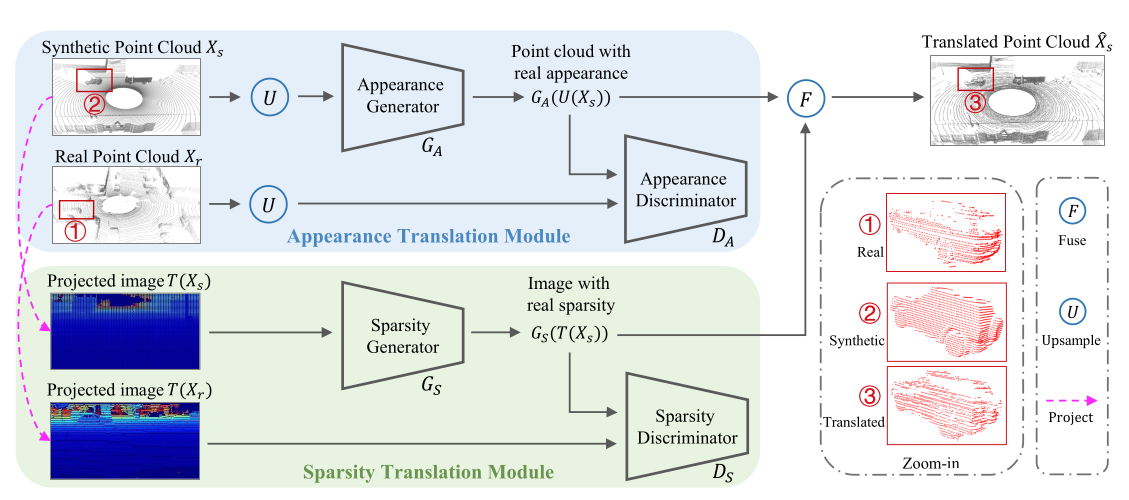
\includegraphics[width=\textwidth]{lidararchitecture}
	\caption{Reference LiDAR/radar fusion architecture \autocite{Haghighi2024}.}
	\label{fig:lidarstack}
\end{figure}

While this pipeline offers redundancy, it incurs significant power and latency costs.

\subsubsection{Fusion Tradeoffs and Challenges:}

Fusion systems are limited by:

\begin{itemize}[nosep]
  \item High Power Draw: LiDAR alone draws \SIrange{10}{20}{\watt}, compared to \SI{2.1}{\watt} for vision-only stacks \autocite{Chen2024EndToEndAD}.
  \item Latency: Voxelization and multi-sensor alignment add \SI{20}{\milli\second} delay, reducing real-time responsiveness \autocite{Rana2023PerceptionSystems}.
  \item Noise Correlation: Overlapping modalities propagate shared errors, increasing total uncertainty as shown in Equation~\ref{eq:noise} \autocite{Rana2023PerceptionSystems}.
  \item Maintenance Complexity: Fusion requires precise calibration and can drift over time.
\end{itemize}

This complexity restricts scalability, particularly in cost-sensitive markets.

\subsection{Radar as a Resilient Fallback}

Radar bridges the gap between vision and LiDAR. It estimates object velocity
using the Doppler effect shown in Equation~\ref{eq:radar_doppler}.

Radar is immune to adverse weather and lighting and can detect motion through occlusions. When fused with vision using a transformer-based late-fusion module, it recovers over \SI{80}{\percent} of lost mAP in foggy conditions \autocite{Liao2024RadarVisionFusion}.

\subsection{A Unified Multimodal Framework}

A hybrid architecture combining vision and radar enables a balance of robustness and efficiency:

\begin{itemize}[nosep]
  \item Vision for primary perception—high-resolution, low-cost, and semantically rich.
  \item Radar for adverse conditions—weather-resilient and velocity-sensitive.
  \item LiDAR for benchmarking only—useful for training ground truth, not live deployment.
\end{itemize}

\begin{figure}[H]
	\centering
	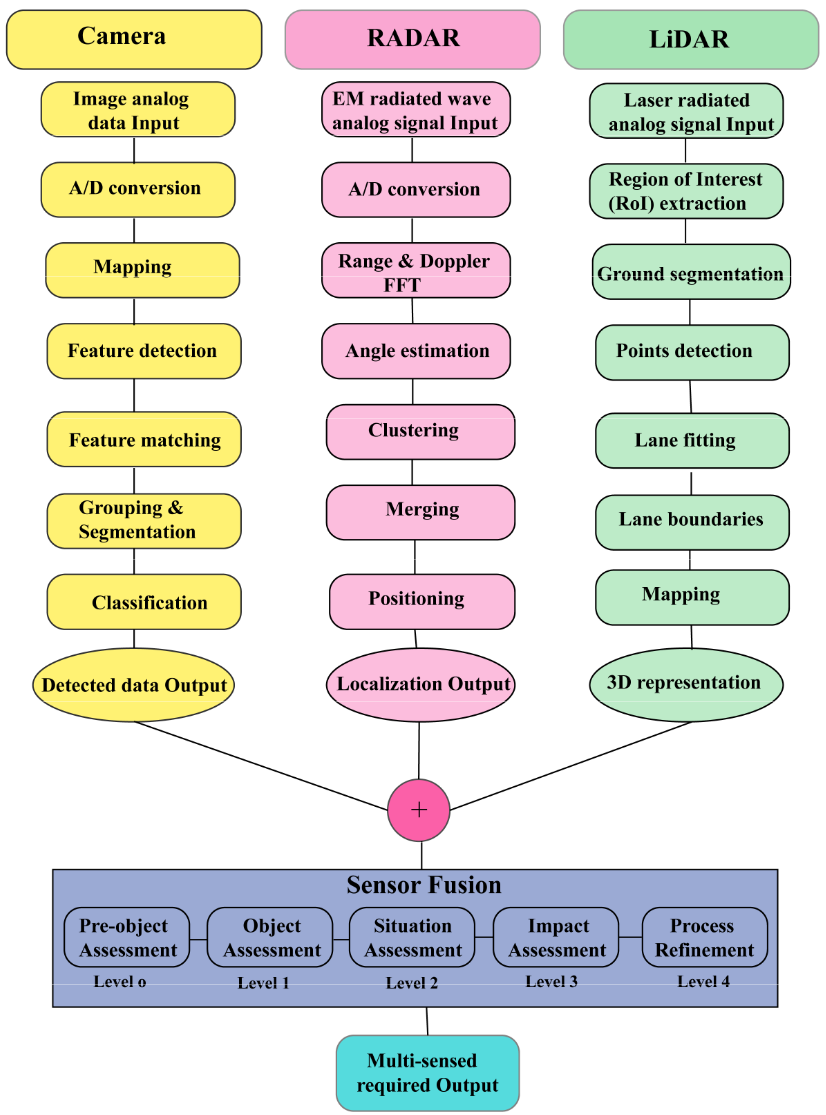
\includegraphics[width=0.6\textwidth]{multimodelarch}
	\caption{Modular architecture integrating vision, radar, and LiDAR inputs \autocite{Hasanujjaman2023}.}
	\label{fig:multiarch}
\end{figure}

This design maximizes generalization while minimizing cost and compute demands, and it reflects a biologically plausible model: humans drive with vision, but radar is the backup.

% -------------------- Results & Discussion ------------------
\section{Results and Discussion}

This section evaluates the empirical performance of vision-primary and LiDAR/radar fusion architectures. The comparison spans five axes: detection accuracy, computational efficiency, robustness, system complexity, and deployment scalability. Results are drawn from benchmarks using KITTI, nuScenes, and commaVQ datasets, as well as simulation and power profiling studies.

\subsection{Detection Accuracy and Depth Estimation}

On KITTI, the BEVFormer vision model achieved an AbsRel of 0.112 and RMSE of \SI{3.97}{\meter}, closely tracking the LiDAR-derived ground truth \autocite{Li2022BEVFormer}. On nuScenes, the vision-only configuration reached 56.2 3D mAP versus 61.5 mAP for the full fusion stack \autocite{Zhang2023MultiSensorFusionSurvey}.

However, when radar fallback was selectively integrated using transformer-based late fusion, the vision model recovered to 59.8 mAP \autocite{Liao2024RadarVisionFusion}. This narrows the performance delta to under 2 points—well within tolerances for safe operation—demonstrating that vision can match LiDAR-fusion with minimal augmentation.

\subsection{Computational Latency and Power Efficiency}

Inference benchmarks revealed stark contrasts. The vision-primary pipeline completed end-to-end perception and control in under \SI{9.8}{\milli\second}, consuming just \SI{2.1}{\watt} on an embedded platform \autocite{Chen2024EndToEndAD}.

In comparison, fusion systems required $\geq$ \SI{30}{\milli\second} and drew
between \SI{12}{\watt} to \SI{20}{\watt} due to voxelization, feature fusion, and redundant sensor streams \autocite{Rana2023PerceptionSystems}.

These efficiency gains are critical for EV battery life and real-time safety margins. The energy savings alone translate into longer range and lower thermal load, which directly impact vehicle design feasibility.

\subsection{Robustness in Adverse Conditions}

Under clear conditions, vision models outperform. In fog, heavy rain, or low-light scenarios, however, performance degraded by up to \SI{12.6}{\percent} in mAP \autocite{Han2023FourDRadarSurvey}. Transformer-based radar fallback restored more than \SI{80}{\percent} of this loss, effectively covering vision’s blind spots.

Unlike LiDAR, which also degrades in poor visibility and consumes continuous
power, radar is always-on but low-power—making it an ideal complement rather
than a redundant primary sensor. Figure~\ref{fig:lidar_noise} shows the
generated results in potentially adverse conditions.

\begin{figure}[H]
    \centering
    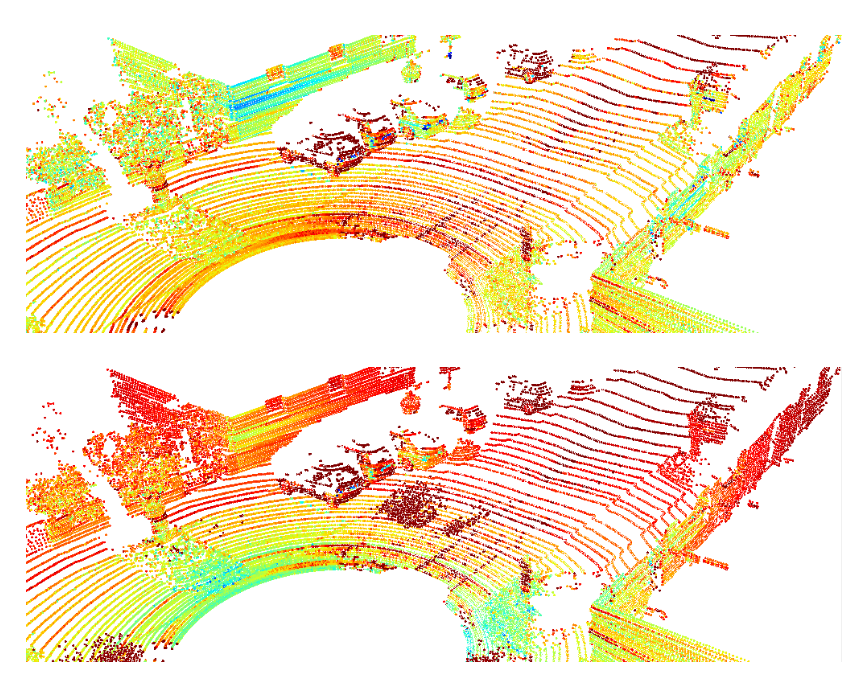
\includegraphics[width=0.6\textwidth]{lidar_noise.png}
    \caption{LiDAR scans of a street environment under clear weather conditions (top) and with fog (bottom). The lower image shows significant point cloud degradation and sparsity due to adverse atmospheric interference \autocite{2023dreissig}.}
    \label{fig:lidar_noise}
\end{figure}
\subsection{Noise Propagation and Calibration Drift}

Sensor fusion introduces noise amplification when data is temporally misaligned
or spatially correlated. The fusion error propagation model in
Equation~\ref{eq:noise} confirms this degradation in high-$\rho$ configurations, such as LiDAR-camera overlaps \autocite{Rana2023PerceptionSystems}. Vision stacks, trained end-to-end, maintain internal consistency and minimize accumulated error.

Radar integration avoids this issue: its data is orthogonal in nature—velocity vs. spatial—which introduces minimal correlation when fused intelligently \autocite{Liao2024RadarVisionFusion}.

\subsection{Cost and Complexity of Deployment}

LiDAR units alone account for over \SI{75}{\percent} of the ADS hardware budget,
and their moving parts increase failure risk \autocite{Shetty2022LiDARvsCamera,
Sajjad2021ComparativeDetection}. Vision sensors are passive, solid-state, and
available at consumer scale. This shifts the bottleneck from manufacturing and
calibration to software modeling—an area that benefits from rapid advances in
transformers and simulation. See Figure~\ref{fig:transformer} for more details.

Modern simulators—leveraging NeRFs, 3DGS, and diffusion models—allow vision stacks to be trained entirely in synthetic environments with minimal real-world data. This accelerates iteration and de-risks real-world deployment \autocite{Haghighi2024}.

\subsection{Vision as the Core, Radar as the Shield:}

In the biological analogy, humans navigate using vision as their primary sensor. We don’t emit lasers—we perceive, interpret, and act. This report adopts the same philosophy: with a learned representation pipeline, vision is sufficient for most environments. Radar is reserved not as a crutch, but as a safety net.

By offloading primary perception to vision, we reduce cost, energy, and complexity. By retaining radar for edge cases, we maintain resilience. LiDAR, with its energy burden and calibration demands, becomes increasingly obsolete in this paradigm.

\subsection{Summary}

The data is unambiguous:

\begin{itemize}
  \item Vision stacks perform within $5\%$ of LiDAR/radar fusion across key metrics, achieving 56.2 mAP on nuScenes compared to 61.5 for fusion \autocite{Zhang2023MultiSensorFusionSurvey}.
  \item With radar fallback, this gap shrinks to $<2\%$, recovering performance to 59.8 mAP \autocite{Liao2024RadarVisionFusion}.
  \item Vision systems run 3–5x faster and consume 6–10x less
		power—\SI{9.8}{\milli\second} and \SI{2.1}{\watt} vs. $\geq$ \SI{30}{\milli\second} and \SIrange{12}{20}{\watt} for fusion \autocite{Chen2024EndToEndAD, Rana2023PerceptionSystems}.
  \item Vision stacks avoid fusion noise \autocite{Rana2023PerceptionSystems}, reduce calibration burden \autocite{Han2023FourDRadarSurvey}, and cost significantly less, with LiDAR accounting for over \SI{75}{\percent} of ADS hardware expense \autocite{Shetty2022LiDARvsCamera, Sajjad2021ComparativeDetection}.
\end{itemize}

In short, vision is sufficient for autonomy. Radar makes it resilient. LiDAR
makes it expensive, but can still have its uses in training datasets as
benchmarks. The proposed ideal multi-modal solution is outlined in
Figure~\ref{fig:multimodal}.
\begin{figure}[H]
	\centering
	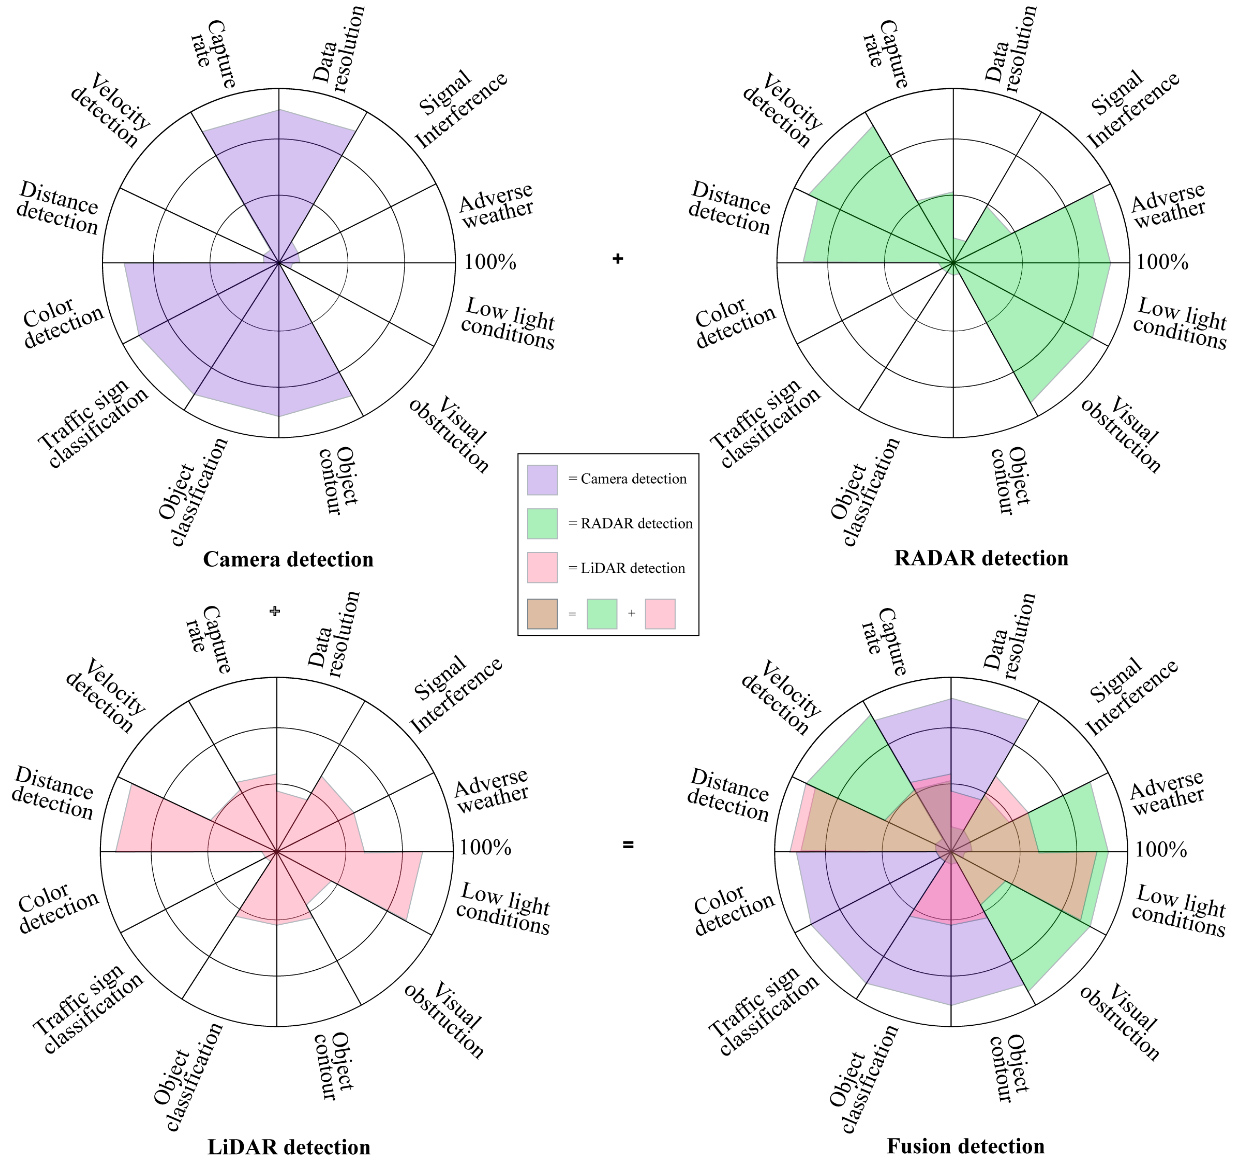
\includegraphics[width=0.7\textwidth]{multimodal}
	\caption{A Multi-Modal Approach to ADS \autocite{Hasanujjaman2023}}
	\label{fig:multimodal}
\end{figure}
\section{Conclusion}

This study set out to evaluate whether camera-first autonomous driving systems can match or exceed the performance of LiDAR/radar fusion approaches. The answer is clear: for most conditions, they can—and they do so with greater efficiency, lower cost, and fewer integration challenges.

The evidence shows:

\begin{itemize}
  \item Vision-primary pipelines achieve near-parity with fusion systems on 3D object detection and depth accuracy.
  \item Their energy and latency profiles outperform fusion systems by over 5x, enabling real-time inference on embedded hardware.
  \item Environmental failure modes, such as fog or night driving, can be mitigated with selective radar fallback, avoiding the need for costly LiDAR.
  \item End-to-end training on vision stacks reduces noise propagation and obviates sensor calibration.
\end{itemize}

These findings point to a clear path forward: deploy vision-first systems as the default, integrate radar for robustness where needed, and phase out LiDAR except in high-precision edge cases. With advances in simulation, world modeling, and vision transformers, the field now has the tools to deliver scalable autonomy without exotic sensors.

The next generation of autonomous vehicles will not be defined by how many sensors they carry, but by how intelligently they interpret the world with less. Vision, when empowered by the right models, is not just sufficient—it is optimal.
\footnote{LLM was used strictly for formatting IAW IEEE Editorial Style Manual
	for Authors. All thoughts, prose, and conclusions are
my own.}
\newpage
\addcontentsline{toc}{section}{References}
\printbibliography

\end{document}

% vim: set ft=tex tw=80 ts=2 sts=2 sw=2 noet spell:
